% Created 2019-01-04 Fri 19:30
% Intended LaTeX compiler: pdflatex
\documentclass[11pt]{article}
\usepackage[utf8]{inputenc}
\usepackage[T1]{fontenc}
\usepackage{graphicx}
\usepackage{grffile}
\usepackage{longtable}
\usepackage{wrapfig}
\usepackage{rotating}
\usepackage[normalem]{ulem}
\usepackage{amsmath}
\usepackage{textcomp}
\usepackage{amssymb}
\usepackage{capt-of}
\usepackage{hyperref}
\author{yeldon}
\date{\textit{[2019-01-04 Fri 17:01]}}
\title{Compile FUNWAVE on Windows 10 ( via Linux Subsystem )}
\hypersetup{
 pdfauthor={yeldon},
 pdftitle={Compile FUNWAVE on Windows 10 ( via Linux Subsystem )},
 pdfkeywords={},
 pdfsubject={},
 pdfcreator={Emacs 25.3.2 (Org mode 9.1.13)}, 
 pdflang={English}}
\begin{document}

\maketitle
\tableofcontents


\section{Preface}
\label{sec:orgd72de78}

The FUNWAVE code is developed with UNIX based operation systems (Linux and OSX).
It used to be easy to compile With Microsoft Windows, but after the MPI feature was
introduced in FUNWAVE, people found diffculties when compiling with Windows OS.
Now, owing to a new feature of Windows 10, called \textbf{Windows Subsystem for Linux},
the FUNWAVE code can be compiled with Windows 10 without annoying
compling rules for windows. The Linux subsystem allows the users to run Linux command in Windows OS. In some sense, the Linux subsystem is similar to the 
virtual machine approach, but it is much easier and much more power than the
virtual machine in the following aspects:

\begin{itemize}
\item fantastic connection between Windows and Linux. You can log in to the Linux
subsystem by simply type bash in windows command window, Besides, one can
get access and write files to \textbf{any} files using the bash commends,
\item No limitation of CPU and RAM.Unlike the virtual machine, Linux system can use
all CPU and RAM of the PC without any restriction.
\end{itemize}

\section{Install Linux Subsystem for Windows 10}
\label{sec:org2fdcf26}

Make sure you have installed Windows 10 and logged in with your Microsoft
account.

The first step is to enable the \textbf{Developer mode} in windows settings

\begin{center}
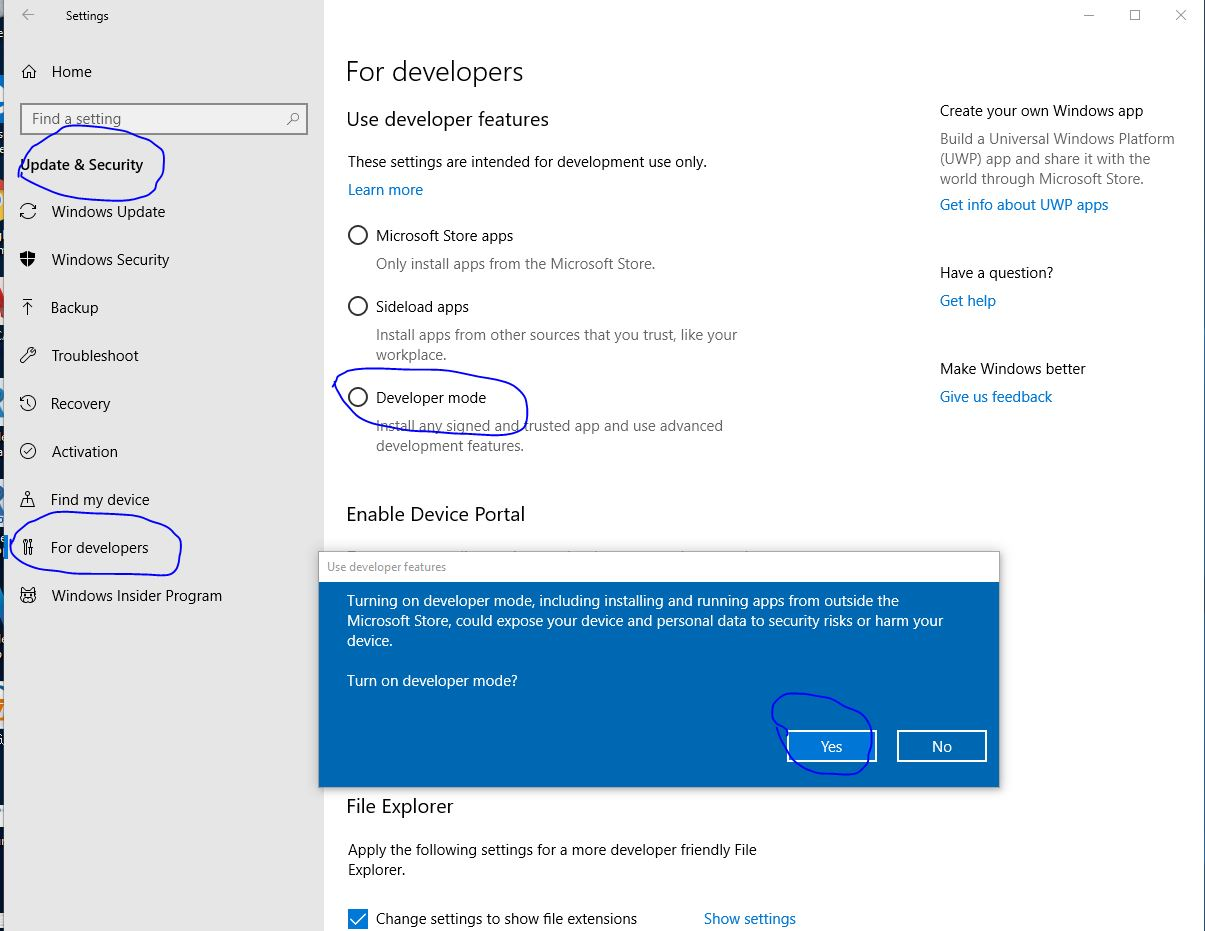
\includegraphics[width=.9\linewidth]{./funwave_img/1.JPG}
\end{center}

Then turn on \textbf{Windows Subsystem for Linux} in \emph{Control Panel}

\begin{center}
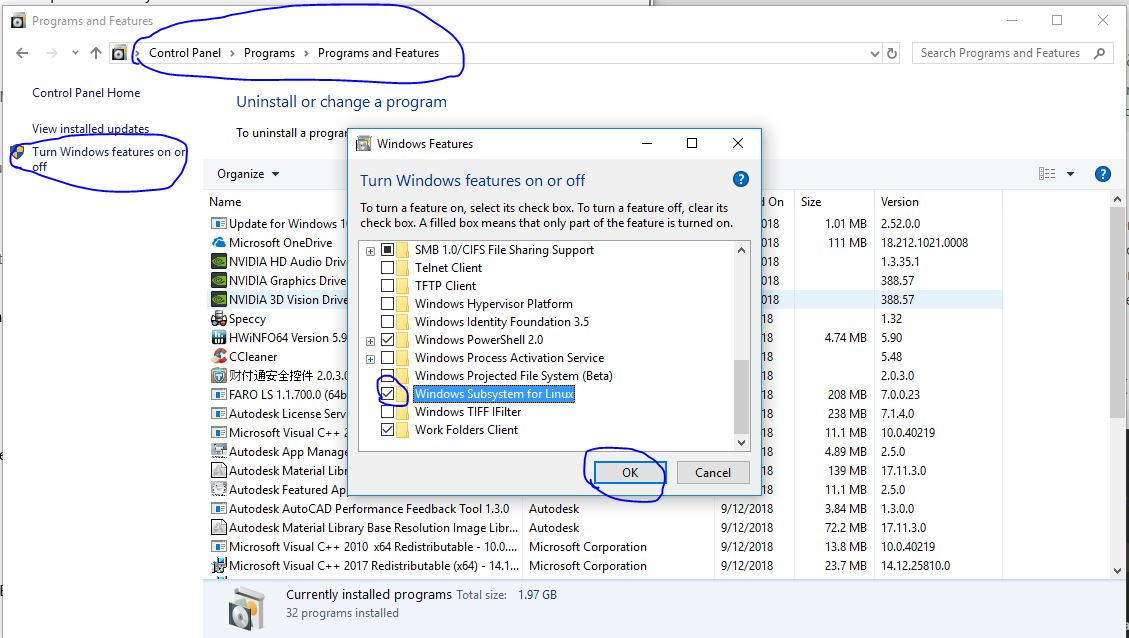
\includegraphics[width=.9\linewidth]{./funwave_img/2.JPG}
\end{center}

Now Download a Linux distribution in \emph{Microsoft Store}. Personally I prefer Ubuntu 16.04 LTS.

\begin{center}
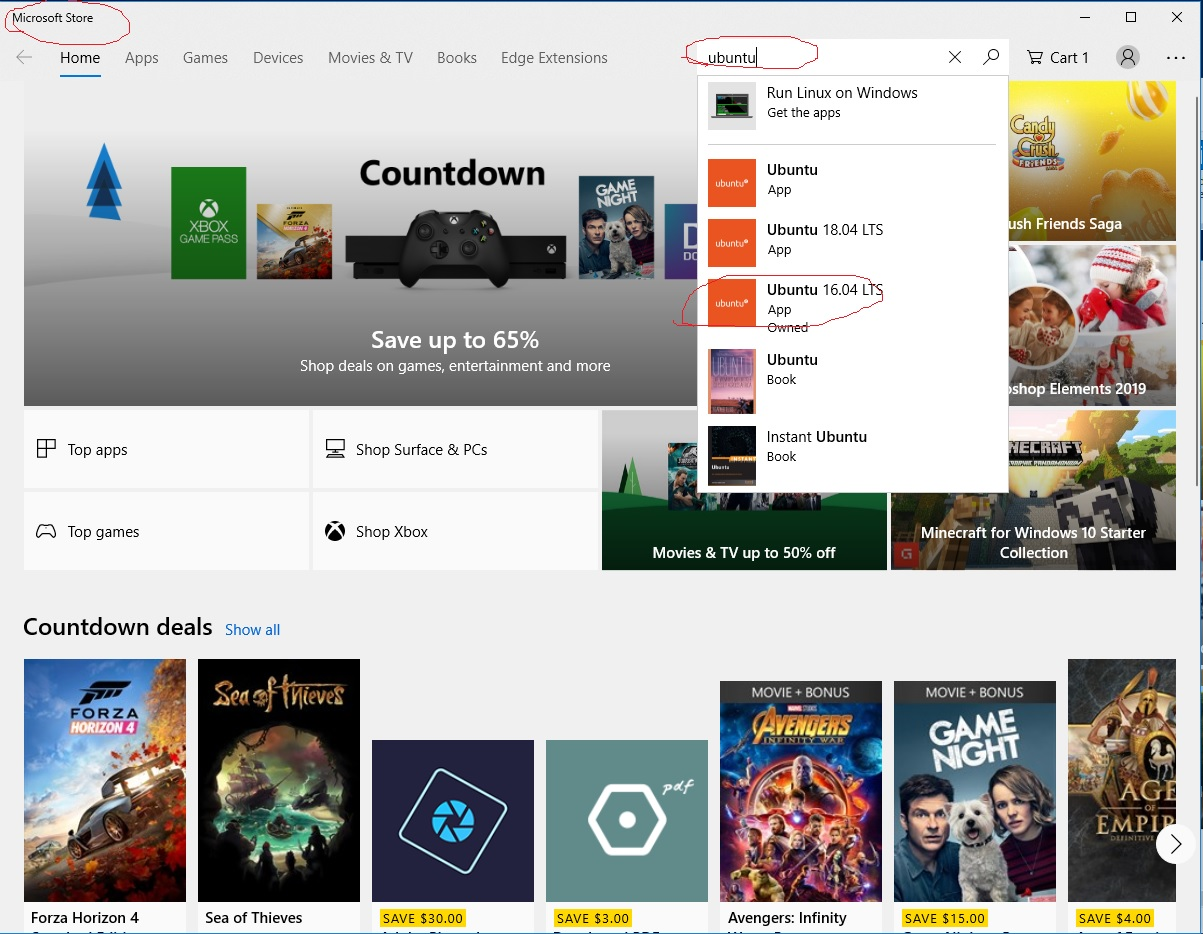
\includegraphics[width=.9\linewidth]{./funwave_img/3.jpg}
\end{center}

After install, you should be able to launch the linux subsystem.

\section{Get ready with Linux Subsytem}
\label{sec:org426a71d}

The first time one launch the Linux subsystem, it takes a couple minutes to
initialization. After the initialization, one would be requested to set the
username and password. 

\begin{center}
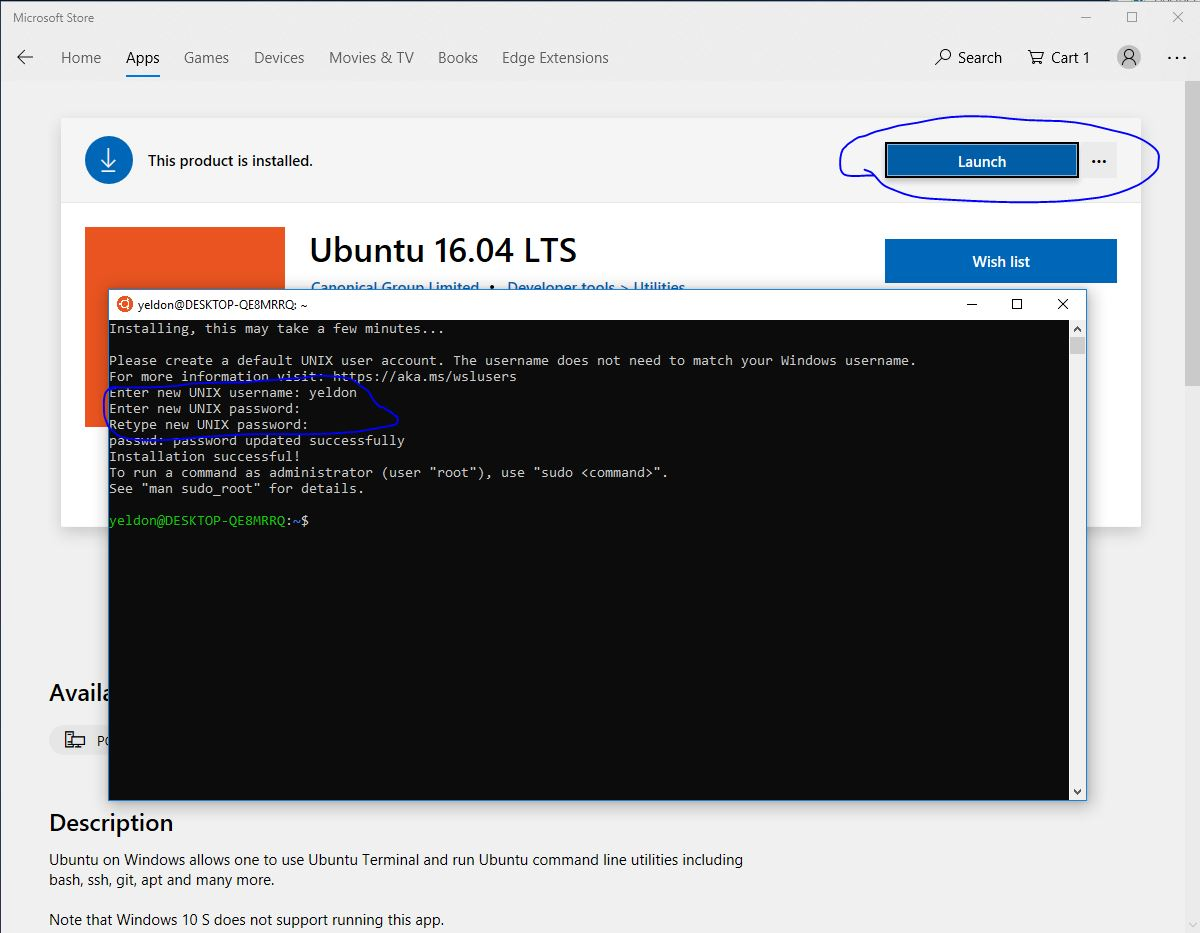
\includegraphics[width=.9\linewidth]{./funwave_img/5.JPG}
\end{center}

type the following commands then you are all set


\begin{verbatim}
sudo apt update
sudo apt upgrade
sudo apt install make
sudo apt install gfortran
sudo apt install mpich
\end{verbatim}

If you are in China, I would remommend you to change the apt source to the
Chinese host. 

\section{Compile and run FUNWAVE}
\label{sec:org970342b}

To lanch the linux subsystem, you can simply run "bash" in \emph{windows command window}, then you are in the real Linux.

It should be noted that you may not get access to all folder. If so, try to get the permission.

\begin{center}
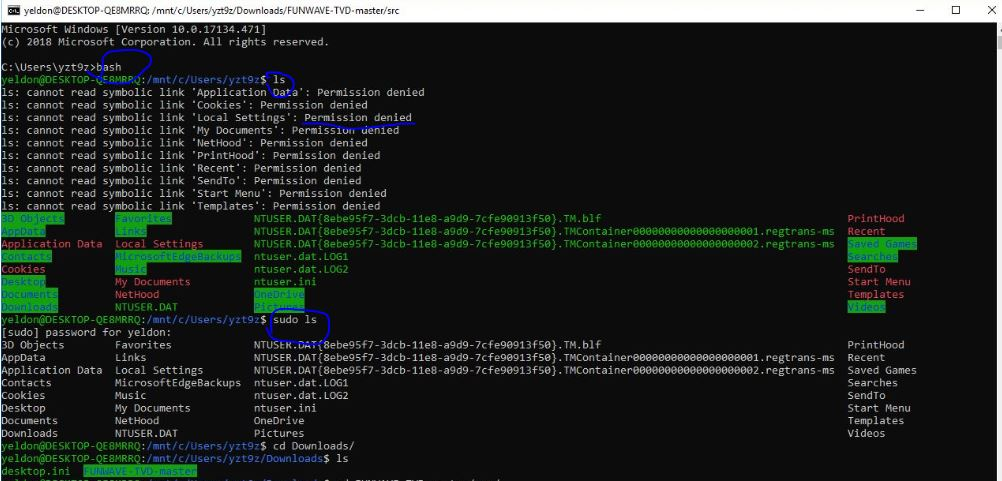
\includegraphics[width=.9\linewidth]{./funwave_img/7.JPG}
\end{center}

With the emaxple \emph{vessel\(_{\text{flat}}\)\(_{\text{bottom}}\)} and set process number as 4, typing 

\begin{verbatim}
make
mpirun -np 4 ./funwave_vessel
\end{verbatim}

The code will be runing in the linux sunsystem. You do not have to worry about
the communication between Linux and Windows, as you can see, as you run the code
in Linux, you can get real-time access to the data files generated by the Linux
excutive.
\begin{center}
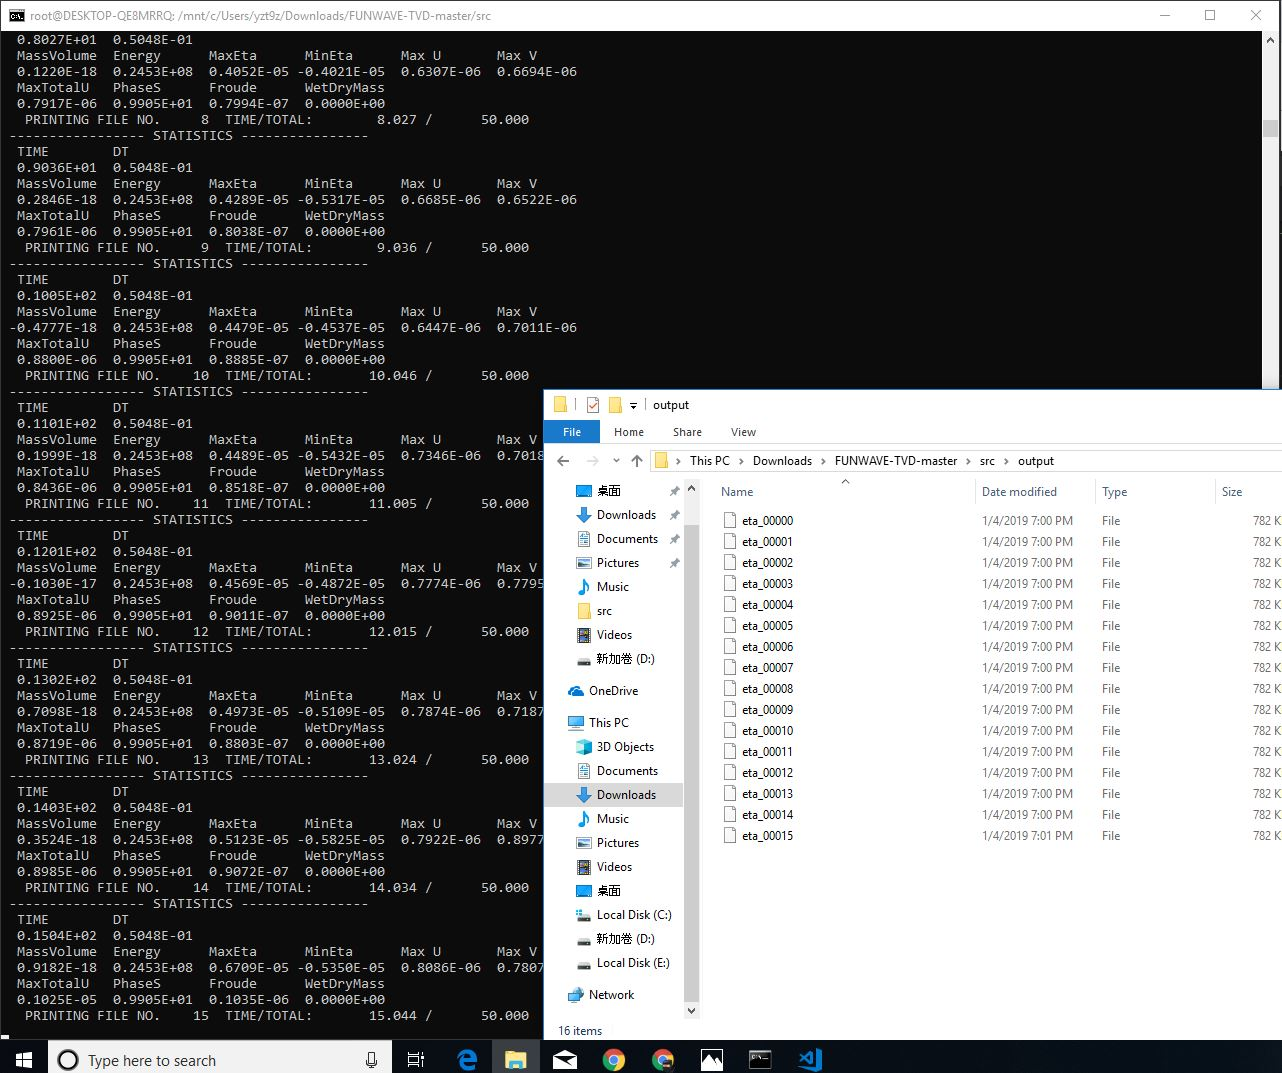
\includegraphics[width=.9\linewidth]{./funwave_img/8.JPG}
\end{center}
\end{document}